\chapter{Introduction}\label{intro}

\section{Clustering}
Clustering\index{Clustering} can be considered as the most important \textit{unsupervised learning} problem;
so, as every other problem of this type, it deals with finding a \textit{structure} in a
collection of given unlabeled datasets. A very common informal definition of clustering could be
``the process of organizing objects into groups whose members are similar in some features of the given dataset".
A \textit{cluster} is therefore a collection of objects which are ``similar" between them and are
``dissimilar" to the objects belonging to other clusters.

We can show this with a simple graphical example:

\begin{figure}[h]
  \centering
  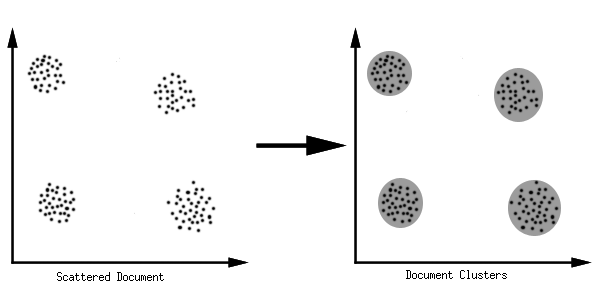
\includegraphics[width=0.9\textwidth]{figures/clustering}
  \caption{Clustering Process}
  \label{fig:clustering}
\end{figure}

In Figure \ref{fig:clustering} we can easily identify the 4 clusters into which the data can be divided; the similarity
criterion is \textit{distance}: two or more objects belong to the same cluster\index{Cluster} if they are ``close" according to a
given distance (in this case geometrical distance). This is called \textit{distance-based clustering}.
Another kind of clustering is \textit{conceptual clustering}: two or more objects belong to the same cluster
if this one defines a concept common to all that objects. In other words, objects are grouped according
to their fit to descriptive concepts, not according to simple similarity measures.

The main goal of clustering is to determine the intrinsic grouping in a given set of unlabeled data.
But there is no such factors to decide what constitutes a good clustering. It can be shown that there is no
absolute ``best" criterion which would be independent of the final aim of the clustering. Consequently, it is the user
which must supply this criterion, in such a way that the result of the clustering will suit their needs.
For instance, we could be interested in finding representatives for homogeneous groups (data reduction),
in finding ``natural clusters"\index{Natural Clusters} and describe their unknown properties (``natural" data types),
in finding useful and suitable groupings (``useful" data classes) or in finding unusual data objects (outlier detection).

\subsection{Applications}
Clustering algorithms can be applied in a very wide range of fields. In \textit{Marketing}\index{Marketing} we can use clustering
to find groups of customers with similar behavior from a large database of customers data containing their properties
and past buying records. In \textit{Biology}\index{Biology} we can classify plants and animals by their given feature sets. Book
ordering and sorting can be a good application of clustering in the \textit{Libraries}\index{Libraries}. \textit{Insurance}\index{Insurance} companies
use clustering for identifying groups of insurance policy holders with a high average claim cost.
Recently urban developers are using clustering methods for identifying groups
of houses according to their house type, value and geographical location in \textit{city-planning}\index{Uraban Planning}. To identify
dangerous zones of earthquake we can observe earthquake epicenters by using clustering algorithms on. These days
clustering algorithms are mostly used in \textit{WWW}\index{World Wide Web} for document classification;
clustering weblog data to discover groups of similar access patterns.

\subsection{Requirements}
The main requirements that a clustering algorithm should satisfy are:
\begin{itemize}
\item \textbf{Scalability} : We need highly scalable clustering algorithms to deal with large databases.
\item \textbf{Ability to deal with different kinds of attributes} : Algorithms should be capable to be applied on any kind of data such as interval-based (numerical) data, categorical, and binary data.
\item \textbf{Discovery of clusters with attribute shape} : The clustering algorithm should be capable of detecting clusters of arbitrary shape. They should not be bounded to only distance measures that tend to find spherical cluster of small sizes.
\item \textbf{High dimensionality} : The clustering algorithm should not only be able to handle low-dimensional data but also the high dimensional space.
\item \textbf{Ability to deal with noisy data} : Databases contain noisy, missing or erroneous data. Some algorithms are sensitive to such data and may lead to poor quality clusters.
\item \textbf{Interpretability} : The clustering results should be interpretable, comprehensible, and usable.
\end{itemize}

\subsection{Problems}
There are a number of problems with clustering. Among them:
\begin{itemize}
\item Current clustering techniques do not address all the requirements adequately (and concurrently);
\item Dealing with large number of dimensions and large number of data items can be problematic because of time complexity;
\item The effectiveness of the method depends on the definition of “distance” (for distance-based clustering);
\item If an obvious distance measure doesn’t exist we must “define” it, which is not always easy, especially in multi-dimensional spaces;
\item The result of the clustering algorithm (that in many cases can be arbitrary itself) can be interpreted in different ways.
\end{itemize}

\subsection{Classification}
Clustering algorithms may be classified as listed below:
\begin{itemize}
\item \textbf{Hierarchical Clustering} : Hierarchical clustering,\index{Hierarchical Clustering} is based on the core idea of objects being more
related to nearby objects than to objects farther away. These algorithms connect ``objects" to form ``clusters"
based on their distance. A cluster can be described largely by the maximum distance needed to connect parts of
the cluster. At different distances, different clusters will form, which can be represented using a \textit{dendrogram},
which explains where the common name ``Hierarchical Clustering" comes from: these algorithms do not provide a
single partitioning of the data set, but instead provide an extensive hierarchy of clusters that merge with each
other at certain distances. In a dendrogram\index{Dendrogram}, the Y-axis marks the distance at which the clusters merge, while the
objects are placed along the X-axis such that the clusters don't mix.

Connectivity based clustering\index{Connectivity Based Clustering} is a whole family of methods that differ by the way distances are computed.
Apart from the usual choice of \textit{distance functions}\index{Distance Functions}, the user also needs to decide on the linkage criterion
(since a cluster consists of multiple objects, there are multiple candidates to compute the distance to) to use.
Popular choices are known as \textit{single-linkage clustering}\index{Single Linkage Clustering} (the minimum of object distances),
\textit{complete linkage clustering}\index{Complete Linkage Clustering} (the maximum of object distances) or UPGMA (``Unweighted Pair Group Method with
Arithmetic Mean"\index{UPGMA}, also known as average linkage clustering)\index{Average Linkage Clustering}. Furthermore, hierarchical clustering can be
agglomerative (starting with single elements and aggregating them into clusters) or divisive
(starting with the complete data set and dividing it into partitions).

\item \textbf{Centroid-based Clustering} : In centroid-based clustering\index{Centroid Based Clustering}, clusters are represented by a central vector,
which may not necessarily be a member of the data set. When the number of clusters is fixed to $K$, $K$-means clustering
gives a formal definition as an optimization problem: find the $K$ cluster centers and assign the objects to the nearest
cluster center, such that the squared distances from the cluster are minimized.

The optimization problem\index{Optimization Problem} itself is known to be NP-hard, and thus the common approach is to search only for approximate
solutions. A particularly well known approximative method is Lloyd's algorithm, often actually referred to as
``$K$-means algorithm". It does however only find a local optimum, and is commonly run multiple times with different
random initializations. Variations of $K$-means\index{K-means} often include such optimizations as choosing the best of multiple runs,
but also restricting the centroids to members of the data set ($K$-medoids)\index{K-medoids}, choosing medians ($K$-medians clustering),
choosing the initial centers less randomly ($K$-means++) or allowing a fuzzy cluster assignment (fuzzy c-means)\index{fuzzy C-means}.

Most $K$-means type algorithms require the number of clusters $K$ to be specified in advance, which is considered
to be one of the biggest drawbacks of these algorithms. Furthermore, the algorithms prefer clusters of approximately
similar size, as they will always assign an object to the nearest centroid. This often leads to incorrectly cut
borders of clusters (which is not surprising since the algorithm optimizes cluster centers, not cluster borders).

\item \textbf{Distribution-based clustering} :\index{Distribution Based Clustering} The clustering model most closely related to statistics is based
on distribution models. Clusters can then easily be defined as objects belonging most likely to the same distribution.
A convenient property of this approach is that this closely resembles the way artificial data sets are generated:
by sampling random objects from a distribution.

While the theoretical foundation of these methods is excellent, they suffer from one key problem known as overfitting\index{Overfitting},
unless constraints are put on the model complexity. A more complex model will usually be able to explain the data better,
which makes choosing the appropriate model complexity inherently difficult.

One prominent method is known as Gaussian mixture models\index{Gaussian Mixture Models} (using the expectation-maximization algorithm). Here,
the data set is usually modelled with a fixed (to avoid overfitting) number of Gaussian distributions that are
initialized randomly and whose parameters are iteratively optimized to better fit the data set. This will converge
to a local optimum, so multiple runs may produce different results. In order to obtain a hard clustering, objects
are often then assigned to the Gaussian distribution they most likely belong to; for soft clusterings, this is not
necessary.

\item \textbf{Density-based Clustering} : In density-based clustering\index{Density Based Clustering}, clusters are defined as areas of higher density
than the remainder of the data set. Objects in these sparse areas that are required to separate clusters are usually
considered to be noise and border points.

The most popular density based clustering method is DBSCAN. In contrast to many newer methods, it features a well-defined
cluster model called ``density-reachability". Similar to linkage based clustering, it is based on connecting points within
certain distance thresholds. However, it only connects points that satisfy a density criterion, in the original variant
defined as a minimum number of other objects within this radius. A cluster consists of all density connected objects
(which can form a cluster of an arbitrary shape, in contrast to many other methods) plus all objects that are within
these objects' range. Another interesting property of DBSCAN is that its complexity is fairly low it requires a linear
number of range queries on the database - and that it will discover essentially the same results (it is deterministic
for core and noise points, but not for border points) in each run, therefore there is no need to run it multiple times.
OPTICS is a generalization of DBSCAN that removes the need to choose an appropriate value for the range parameter ${\varepsilon}$,
and produces a hierarchical result related to that of linkage clustering. DeLi-Clu, Density-Link-Clustering\index{Density Link Clustering} combines ideas
from single-linkage clustering and OPTICS, eliminating the ${\varepsilon}$ parameter entirely and offering performance improvements
over OPTICS by using an R-tree index.

The key drawback of DBSCAN\index{DBSCAN} and OPTICS\index{OPTICS} is that they expect some kind of density drop to detect cluster borders.
On data sets with, for example, overlapping Gaussian distributions a common use case in artificial data the
cluster borders produced by these algorithms will often look arbitrary, because the cluster density decreases
continuously. On a data set consisting of mixtures of Gaussians, these algorithms are nearly always outperformed
by methods such as EM clustering that are able to precisely model this kind of data.
\end{itemize}

\section{Literature Survey}

\subsection{Values of $K$ specified within a range or set}
The  performance  of  a  clustering  algorithm  may  be
affected by the chosen value of $K$. Therefore, instead
of using a single predefined $K$, a set of values might
be   adopted.   It   is   important   for   the   number   of
values  considered  to  be  reasonably  large,  to  reflect
the  specific  characteristics  of  the  data  sets.  At  the
same  time,  the  selected  values  have  to  be  significantly
smaller  than  the  number  of  objects  in  the
data sets, which is the main motivation for performing data clustering.

Reported studies~\cite{han00, daoud95, daoud96, ranka98, bilmes97, bengio95}
on $K$-means clustering and
its  applications  usually  do  not  contain  any  explanation
or  justification  for  selecting  particular  values for $K$.
First,  a  number  of  researchers~\cite{bilmes97, bengio95} used  only  one  or  two  values  for $K$.
Second, several  other  researchers~\cite{han00, daoud96} utilized relatively  large $K$
values  compared  with  the  number of  objects.  These  two  actions  contravene
the  above mentioned  guidelines  for  selecting $K$. Therefore,the
clustering  results  do  not  always  correctly  represent
the performance of the tested algorithms.

In  general,  the  performance  of  any  new  version
of the $K$-means algorithm could be verified by comparing  it  with  its  predecessors  on  the  same  criteria.
In   particular,   the   sum   of   cluster   distortions   is
usually  employed  as  such  a  performance  indicator.~\cite{daoud96, bengio95}
Thus, the comparison is considered fair  because  the  same  model and  criterion  are  used
for the performance analysis.

\subsection{Values of $K$ specified by the user}
The $K$-means  algorithm  implementation  in  many
data-mining   or   data   analysis   software   packages~\cite{hall02}
requires the number of clusters to be specified
by  the  user.  To  find  a  satisfactory  clustering
result,  usually,  a  number  of  iterations  are  needed
where the user executes the algorithm with different
values  of $K$.  The  validity  of  the  clustering  result  is
assessed  only  visually  without  applying  any  formal
performance   measures.   With   this   approach,   it   is
difficult  for  users  to  evaluate  the  clustering  result
for multi-dimensional data sets.

\subsection{Values of $K$ determined in a later processing step}
When $K$-means clustering is used as a pre-processing
tool,  the  number  of  clusters  is  determined  by  the
specific requirements of the main processing algorithm.~\cite{hansen96}
No  attention  is  paid  to  the  effect  of
the  clustering  results  on  the  performance  of  this
algorithm. In such applications, the $K$-means
algorithm  is  employed  just  as  a  `black  box'  without
validation of the clustering result.

\subsection{Values of $K$ equated to the number of generators}
Synthetic   data   sets,   which   are   used   for   testing
algorithms,  are  often  created  by  a  set  of  normal  or
uniform   distribution   generators.   Then,   clustering
algorithms  are  applied  to  those  data  sets  with  the
number of clusters equated to the number of generators.
It  is  assumed  that  any  resultant  cluster  will
cover  all  objects  created  by  a  particular  generator.
Thus,  the  clustering  performance  is  judged  on  the
basis  of  the  difference  between  objects  covered  by
a  cluster  and  those  created  by  the  corresponding
generator.  Such  a  difference  can  be  measured  by
simply   counting   objects   or   calculating   the
information gain.~\cite{bradly98}

Unfortunately,  this  method  of  selecting $K$ cannot
be  applied  to  practical  problems.  The  data  distribution
in  practical  problems  is  unknown  and  also
the number of generators cannot be specified.

\subsection{Values of $K$ determined by statistical measures}
There  are  several  statistical  measures  available  for
selecting $K$. These measures are often applied in combination
with   probabilistic   clustering   approaches.
They are calculated with certain assumptions
about  the  underlying  distribution  of  the  data.  The
Bayesian   information   criterion\index{Bayesian Information Criterion}   or   Akeike’s   information~\cite{ishioka00}
criterion  is  calculated  on  data  sets
which  are  constructed  by  a  set  of  Gaussian  distributions.
The  measures  applied  by  Hardy  are
based  on  the  assumption  that  the  data  set  fits  the
Poisson distribution. Monte Carlo techniques,\index{Monte Carlo}
which  are  associated  with  the null  hypothesis\index{Null Hypothesis},  are
used for assessing the clustering results and also for
determining the number of clusters.

\subsection{Values of $K$ determined through visualization}
Visual  verification  is  applied  widely  because  of  its
simplicity and explanation possibilities. Visual
examples  are  often  used  to  illustrate  the  drawbacks
of an algorithm or to present the expected clustering
results.~\cite{bilmes97}

The    assessment    of    a    clustering    result    using
visualization  techniques  depends  heavily  on  their
implicit  nature.  The  clustering  models  utilized  by
some  clustering  methods  may  not  be  appropriate
for   particular   data   sets. The  application  of
visualization  techniques  implies  a  data  distribution
continuity  in  the  expected  clusters.  If  the $K$-means
approach  is  applied  to  such  data  sets,  there  is  not
any    cluster    that    satisfies   the $K$-means   clustering
model  and  at  the  same  time  corresponds  to  a
particular   object   grouping   in   the   illustrated   data
sets.  Therefore,  the $K$-means  algorithm  cannot  produce
the  expected  clustering  results.  This  suggests
that  the $K$-means  approach  is  unsuitable  for  such
data sets.

\section{Objective}
Partitioning methods or Centroid-base Clustering algorithms, such as $K$-means clustering require the users to specify
the number of clusters to be generated. One fundamental question is: If the data is clusterable, then how to choose the
right number of expected clusters $K$? Unfortunately, there is no definitive answer to this question. The optimal
clustering is somehow subjective and depend on the method used for measuring similarities and the parameters used for
partitioning.

In this work, our prime objectives are:

\begin{itemize}
\item Describing different methods of determining the optimal number of clusters for $K$-means clustering.
\item These methods include direct methods and statistical testing methods. Direct methods consists of
optimizing a criterion, such as the within cluster sums of squares or the average silhouette. Statistical
testing methods consists of comparing evidence against null hypothesis. An example is the gap statistic.
\item We'll apply these methods on various data sets and find the optimal number of clusters for $K$-means clustering.
\item Finally we'll compare performance among these methods on the basis of determining number of clusters for
different data sets.
\end{itemize}

\section{Thesis Organization}
In Chapter One, we try to give a general overview about what is machine learning, clustering,
why clustering is so important and what are the factors behind determining number of clusters.
In Chapter Two, we will discuss the idea behind determining number of clusters of a dataset and
how it affects the output of $K$-means algorithm.
In Chapter Three, we will describe different methods for selecting number of clusters and there approach,
algorithms.
In Chapter Four, we want to show experimental result of our reviewed methods algorithm and output.
Then we'll compare the output with the original output.
In Chapter Five, we put a discussion about the future of this work, where it can give promising
result and how it can be improved further.

\endinput
